\documentclass[../../main.tex]{subfiles}

\begin{document}
\chapter{Krylov Subspaces}\label{chap:krylov}

Krylov subspaces capture the span of repeated applications of a matrix to a vector and are the foundation of projection methods driven by matrix--vector products.

\begin{definition}{Krylov subspace}{krylov}
  For $A\in\mathbb{R}^{n\times n}$ and a nonzero $\mathbf{v}\in\mathbb{R}^n$, the $m$-th Krylov subspace is
  \[
    \mathcal{K}_m(A,\mathbf{v}) := \operatorname{span}\{\mathbf{v},A\mathbf{v},A^2\mathbf{v},\ldots,A^{m-1}\mathbf{v}\}.
  \]
  Always $\dim\,\mathcal{K}_m\le \min\{m,n\}$.
\end{definition}

\section{Properties of Krylov Subspaces}
\label{sec:properties-krylov-subspaces}

\subsection{Minimal polynomial and grade}
The \emph{grade} $\mu$ of $\mathbf{v}$ with respect to $A$ is the degree of the monic polynomial $p$ of least degree such that $p(A)\mathbf{v}=0$. Then
\[
  A\mathcal{K}_\mu(A,\mathbf{v}) = \mathcal{K}_\mu(A,\mathbf{v}),\qquad \mathcal{K}_m(A,\mathbf{v})=\mathcal{K}_\mu(A,\mathbf{v})\;\text{for all }m\ge \mu.
\]
Thus Krylov spaces stabilize once an $A$-invariant subspace is reached (\texttt{happy breakdown}).

\paragraph{Cayley--Hamilton} For any $\mathbf{x}\in\mathcal{K}_m(A,\mathbf{v})$ with $m\ge\mu$, there exists a polynomial $q_{\mu-1}$ of degree at most $\mu-1$ such that
\[
  \mathbf{x}=q_{\mu-1}(A)\,\mathbf{v}.
\]
Indeed, dividing any polynomial representative by the minimal polynomial gives $q=q_1\,p+q_{\mu-1}$ and $q(A)\mathbf{v}=q_{\mu-1}(A)\mathbf{v}$.

\paragraph{Dimension and nesting.} The dimensions satisfy
\[
  \dim\mathcal{K}_m(A,\mathbf{v}) \le m,\qquad \mathcal{K}_1\subseteq\mathcal{K}_2\subseteq\cdots\subseteq\mathcal{K}_\mu=\cdots.
\]

\paragraph{Projection viewpoint.} Given an initial guess $\mathbf{x}_0$ for $A\mathbf{x}=\mathbf{b}$ and residual $\mathbf{r}_0$, Krylov methods search in $\mathbf{x}_0+\mathcal{K}_m(A,\mathbf{r}_0)$ while enforcing a Petrov--Galerkin condition on the residual. Choices of the test space $\mathcal{L}$ produce FOM ($\mathcal{L}=\mathcal{K}_m$) and GMRES ($\mathcal{L}=A\mathcal{K}_m$); see Chapters~\ref{chap:arnoldi} and \ref{chap:projection-methods}.

\section{Arnoldi Iteration}
\label{sec:arnoldi-iteration}
The \emph{Arnoldi iteration} is a \emph{Krylov subspace iterative method} that reduces $A$ to an \textbf{upper Hessenberg matrix} $H_m$.
We can then use this simple representation of $A$ to approximate some \textbf{eigenvalues} of $A$.

\subsection{Derivation of Arnoldi Iteration}
Let $A \in \mathbb{C}^{n \times n}$.
We want to compute $A = V H V^\ast$ where $H$ is upper Hessenberg and $V$ is unitary ($V^\ast V = I$).

\paragraph{But why do we want to compute $A = V H V^\ast$?}
The reason is that such a \emph{unitary similarity} preserves the eigenvalues of $A$, while making the matrix $H$ much simpler in structure (upper Hessenberg).
Indeed, since $H = V^\ast A V$, if $H\mathbf{x} = \lambda \mathbf{x}$, then
\[
  A(V\mathbf{x}) = V H \mathbf{x} = \lambda (V\mathbf{x}),
\]
so $A$ and $H$ share the same eigenvalues.

\paragraph{But what if $A$ is very large?}
For $n \gg 1$, computing the full factorization is too expensive and unnecessary.
Instead, we work with a smaller subspace of dimension $m \ll n$.

\[
  A V_m \approx V_m H_m,
\]

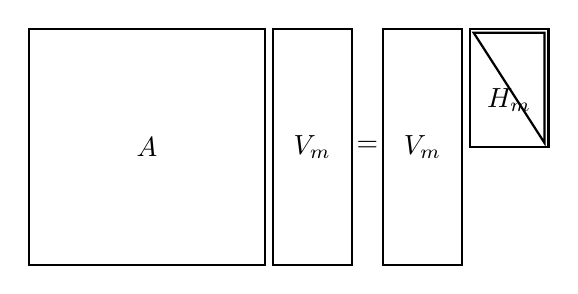
\begin{tikzpicture}
  % n x n square representing A
  \draw[thick] (0, 0) rectangle (3, 3);
  \node at (1.5, 1.5) {$A$};
  % n x m rectangle representing V_m
  \draw[thick] (3.1, 0) rectangle (4.1, 3);
  \node at (3.6, 1.5) {$V_m$};
  % =
  \node at (4.3, 1.5) {$=$};
  % n x m rectangle representing V_m
  \draw[thick] (4.5, 0) rectangle (5.5, 3);
  \node at (5, 1.5) {$V_m$};
  % m x m square representing H_m
  \draw[thick] (5.6, 1.5) rectangle (6.6, 3);
  % Triangle to indicate upper Hessenberg
  \draw[thick] (5.65, 2.95) -- (6.55, 2.95) -- (6.55, 1.55) -- cycle;
  \node at (6.1, 2.1) {$H_m$};
\end{tikzpicture}

Consider the sequence of vectors generated by repeatedly applying a matrix $A$ to an initial vector $\mathbf{r}_0$:
\[
  \mathbf{r}_0, \quad A\mathbf{r}_0, \quad A^2\mathbf{r}_0, \quad A^3\mathbf{r}_0, \quad \ldots
\]

The \emph{Krylov subspace} of dimension $m+1$ is the span of the first $m+1$ such vectors:
\[
  \mathcal{K}_{m+1}(A,\mathbf{r}_0) := \text{span}\{\mathbf{r}_0, A\mathbf{r}_0, A^2\mathbf{r}_0, \ldots, A^m\mathbf{r}_0\}
\]

While this sequence captures how $A$ acts on $\mathbf{r}_0$, these vectors typically become increasingly aligned and numerically dependent. The Arnoldi process transforms this unwieldy sequence into an orthonormal basis that preserves all the essential information about $A$'s action on the Krylov subspace.


\subsection{The Arnoldi Algorithm}
The key insight of Arnoldi iteration is to apply the Gram-Schmidt process \emph{incrementally} as we build up the Krylov subspace. Starting with $\mathbf{v}_1 = \mathbf{r}_0/\|\mathbf{r}_0\|_2$, we:


\begin{algorithm}[htbp]
  \caption{Arnoldi Iteration (Modified Gram-Schmidt)}
  \label{alg:arnoldi}
  \begin{algorithmic}
    \Require $A\in\mathbb{R}^{n\times n}$, $\mathbf{b}\in\mathbb{R}^n$, $\mathbf{x}_0$ (init. guess), $m$ (num. steps)
    \Ensure  $V_{m+1} = [\mathbf{v}_1, \ldots, \mathbf{v}_{m+1}]$ (Orth. basis of $\mathcal{K}_{m+1}$, $n\times m$), $\overline{H}_m$ (Upper Hessenberg, $(m+1)\times m$)
    \State $\mathbf{r}_0 \gets \mathbf{b} - A\mathbf{x}_0$, $\beta \gets \|\mathbf{r}_0\|_2$, $\mathbf{v}_1 \gets \mathbf{r}_0/\beta$
    \For{$j = 1, 2, \ldots, m$}
    \State $\mathbf{w}_j \gets A\mathbf{v}_j$
    \For{$i = 1, 2, \ldots, j$}
    \State $h_{i,j} \gets \langle\mathbf{v}_i, \mathbf{w}_j\rangle$
    \State $\mathbf{w}_j \gets \mathbf{w}_j - h_{i,j}\mathbf{v}_i$
    \EndFor
    \State $h_{j+1,j} \gets \|\mathbf{w}_j\|_2$
    \If{$h_{j+1,j} = 0$}
    \State \textbf{Break}
    \EndIf
    \State $\mathbf{v}_{j+1} \gets \mathbf{w}_j/h_{j+1,j}$
    \EndFor
  \end{algorithmic}
\end{algorithm}

After $m$ steps, we have constructed:
\begin{align}
  V_{m+1}        & = [\mathbf{v}_1, \mathbf{v}_2, \ldots, \mathbf{v}_{m+1}] \in \mathbb{R}^{n \times (m+1)} \quad \text{(orthonormal basis)} \\
  V_m            & = [\mathbf{v}_1, \mathbf{v}_2, \ldots, \mathbf{v}_m] \in \mathbb{R}^{n \times m} \quad \text{(first $m$ columns)}         \\
  \overline{H}_m & = \begin{bmatrix}
                       h_{1,1} & h_{1,2} & h_{1,3} & \cdots  & h_{1,m}   \\
                       h_{2,1} & h_{2,2} & h_{2,3} & \cdots  & h_{2,m}   \\
                       0       & h_{3,2} & h_{3,3} & \cdots  & h_{3,m}   \\
                       \vdots  & \ddots  & \ddots  & \ddots  & \vdots    \\
                       0       & \cdots  & 0       & h_{m,m} & h_{m,m}   \\
                       0       & \cdots  & 0       & 0       & h_{m+1,m}
                     \end{bmatrix} \in \mathbb{R}^{(m+1) \times m}
\end{align}
The matrix $\overline{H}_m$ is \emph{upper Hessenberg} (zero below the first subdiagonal) and encodes all the orthogonalization coefficients from the Gram-Schmidt process.

\subsection{Arnoldi Relation}
The fundamental relationship is:
\begin{align*}\label{eq:arnoldi-relation}
  AV_m & = V_{m+1}\overline{H}_m = V_m H_m + h_{m+1,m}\mathbf{v}_{m+1}\mathbf{e}_m^T \\
  H_m  & = V_m^\top A V_m
\end{align*}

This compact relation captures a profound fact: \emph{the action of the large matrix $A$ on the Krylov subspace is completely characterized by the small Hessenberg matrix $\overline{H}_m$}.
Column by column, this says:
\[
  A\mathbf{v}_j = h_{1,j}\mathbf{v}_1 + h_{2,j}\mathbf{v}_2 + \cdots + h_{j,j}\mathbf{v}_j + h_{j+1,j}\mathbf{v}_{j+1}
\]
In other words, $A\mathbf{v}_j$ lies in $\text{span}\{\mathbf{v}_1, \ldots, \mathbf{v}_{j+1}\}$, which is exactly what we'd expect since $A\mathbf{v}_j$ is the $(j+1)$-th Krylov vector (before orthogonalization).

\subsection{Breakdown Conditions}
If $h_{j+1,j} = 0$ for some $j < m$, then $\mathbf{w} = A\mathbf{v}_j$ lies entirely in $\text{span}\{\mathbf{v}_1, \ldots, \mathbf{v}_j\}$. This means:
\[
  A(\mathcal{K}_j(A,\mathbf{r}_0)) \subseteq \mathcal{K}_j(A,\mathbf{r}_0)
\]
The Krylov subspace is \emph{$A$-invariant}, and we have found an exact invariant subspace. This is called "happy breakdown" because:
\begin{itemize}
  \item We can solve linear systems exactly within this subspace
  \item We have found exact eigenvalue/eigenvector information
  \item No further iteration is needed
\end{itemize}

\paragraph{Near-breakdown.}
In finite precision arithmetic, $h_{j+1,j}$ may be very small but nonzero, leading to numerical instability. This requires careful handling through techniques like deflation or restarting.

\subsection{Numerical Stability and Reorthogonalization}
The Modified Gram-Schmidt process used in Algorithm~\ref{alg:arnoldi} is more numerically stable than Classical Gram-Schmidt, but orthogonality can still be lost due to:
\begin{itemize}
  \item Round-off errors accumulating over many iterations
  \item Nearly linearly dependent Krylov vectors
  \item Ill-conditioned matrices $A$
\end{itemize}

\subsection{Computational Complexity}

\paragraph{Per iteration cost:}
\begin{itemize}
  \item One matrix-vector product: $A\mathbf{v}_j$ costs $O(\text{nnz}(A))$ or $O(n^2)$ flops
  \item Orthogonalization: $j$ inner products and $j$ vector updates cost $O(jn)$ flops
\end{itemize}

\paragraph{Total cost for $m$ iterations:}
\[
  \text{Flops} = O\left(m \cdot \text{cost}(A\mathbf{v}) + \sum_{j=1}^m jn\right) = O(m \cdot \text{cost}(A\mathbf{v}) + m^2n)
\]

\paragraph{Storage requirements:}
\begin{itemize}
  \item Basis vectors $V_{m+1}$: $O(nm)$ memory
  \item Hessenberg matrix $\overline{H}_m$: $O(m^2)$ memory
  \item \textbf{Total}: $O(nm + m^2)$ memory
\end{itemize}

The storage requirement $O(nm)$ can become prohibitive for large $m$, motivating restarted variants.

\subsection{Applications: The Foundation for Krylov Solvers}

The Arnoldi relation \eqref{eq:arnoldi-relation} enables two major classes of iterative solvers:

\paragraph{Full Orthogonalization Method (FOM):}
Uses Galerkin projection: find $\mathbf{x}_m \in \mathbf{x}_0 + \mathcal{K}_m(A,\mathbf{r}_0)$ such that the residual is orthogonal to the Krylov subspace.

\paragraph{Generalized Minimal Residual (GMRES):}
Uses minimal residual projection: find $\mathbf{x}_m \in \mathbf{x}_0 + \mathcal{K}_m(A,\mathbf{r}_0)$ that minimizes $\|A\mathbf{x}_m - \mathbf{b}\|_2$.

Both methods reduce the original $n \times n$ problem to an $m \times m$ problem involving $H_m$ or $\overline{H}_m$.

\begin{summary}{The Power of Arnoldi}{arnoldi-summary}
  The Arnoldi iteration transforms the numerically unstable sequence $\{\mathbf{r}_0, A\mathbf{r}_0, A^2\mathbf{r}_0, \ldots\}$ into:
  \begin{itemize}
    \item A numerically stable orthonormal basis $V_{m+1}$ of $\mathcal{K}_{m+1}(A,\mathbf{r}_0)$
    \item A compact representation $\overline{H}_m$ of how $A$ acts on the Krylov subspace
    \item The fundamental relation $AV_m = V_{m+1}\overline{H}_m$ that enables efficient projections
    \item A foundation for optimal Krylov subspace methods like GMRES
    \item Natural stopping criteria through happy breakdown detection
  \end{itemize}
  This combination of numerical stability, dimensional reduction, and preserved spectral information makes Arnoldi iteration one of the most important algorithms in numerical linear algebra.
\end{summary}

The specific applications of this framework to solve linear systems and eigenvalue problems are developed in Chapter~\ref{chap:projection-methods}, where we'll see how the Arnoldi relation enables both exact solutions (via FOM) and optimal approximations (via GMRES).


\section{Lanczos Iteration}
\label{sec:lanczos-iteration}

When $A=A^\top$ is symmetric, the Arnoldi process simplifies to the \emph{Lanczos iteration}, which produces a tridiagonal matrix $T_m$ instead of a Hessenberg matrix $\overline{H}_m$.

\subsection{Derivation of Lanczos Iteration}
We first start with the assumption that $A$ is \emph{symmetric and positive definite} (SPD), i.e., $A = A^T \succ 0$.

Then we have the Arnoldi relation
\begin{align*}
  AV_m = V_{m+1}\overline{H}_m \\
  H_m = V_m^\top A V_m
\end{align*}
Where we solve the reduced linear system:
\begin{align*}
  \mathbf{x}_m & = \mathbf{x}_0 + V_m H_m^{-1} V_m^\top \mathbf{r}_0                                \\
               & = \mathbf{x}_0 + V_m H_m^{-1} \beta \mathbf{e}_1, \quad \beta = \|\mathbf{r}_0\|_2 \\
  \mathbf{x}_m & = \mathbf{x}_0 + V_m \mathbf{y}_m
\end{align*}

\textit{How can this be simplified if $A = A^\top$?}
In this case $H_m = V_m^\top A V_m = H_m^\top$ is symmetric, and since it is upper Hessenberg it must be tridiagonal.
$H_m$ is then tridiagonal and symmetric, i.e., $H_m$ has the form:
\[
  H_m =
  \begin{bmatrix}
    \alpha_1 & \beta_2  & 0       & \cdots  & 0        \\
    \beta_2  & \alpha_2 & \beta_3 & \cdots  & 0        \\
    0        & \beta_3  & \ddots  & \ddots  & \vdots   \\
    \vdots   & \vdots   & \ddots  & \ddots  & \beta_m  \\
    0        & 0        & 0       & \beta_m & \alpha_m
  \end{bmatrix}
\]

\begin{algorithm}[htbp]
  \caption{Lanczos Iteration (Arnoldi for symmetric $A=A^\top$)}
  \label{alg:lanczos}
  \begin{algorithmic}[0]
    \Require $A, \mathbf{b}, \mathbf{x}_0, m$
    \State $\beta_1 = 0$
    \State $\mathbf{v}_0 = 0$
    \State $\mathbf{r}_0 = \mathbf{b} - A\mathbf{x}_0$
    \State $\beta = \|\mathbf{r}_0\|_2$
    \State $\mathbf{v}_1 = \dfrac{\mathbf{r}_0}{\beta}$
    \For{$j = 1, 2, \ldots, m$}
    \State $\mathbf{w}_j = A\mathbf{v}_j - \beta_j \mathbf{v}_{j-1}$, where $\beta_1 \mathbf{v}_0 = 0$
    \State $\alpha_j = \langle \mathbf{w}_j, \mathbf{v}_j \rangle$
    \State $\mathbf{w}_j = \mathbf{w}_j - \alpha_j \mathbf{v}_j$
    \State $\beta_{j+1} = \|\mathbf{w}_j\|_2$
    \If{$\beta_{j+1} = 0$} \textbf{Stop}
    \EndIf
    \State $\mathbf{v}_{j+1} = \frac{\mathbf{w}_j}{\beta_{j+1}}$
    \EndFor
    \Return $V_{m+1} = [\mathbf{v}_1, \ldots, \mathbf{v}_{m+1}]$
    \State $T_m = \operatorname{tridiag}(\beta_i, \alpha_i, \beta_{i+1}), \quad i=1,\ldots,m$
    \State $\mathbf{x}_m = \mathbf{x}_0 + V_m T_m^{-1} \beta \mathbf{e}_1$
    \State \textbf{Solve:} $T_m \mathbf{y}_m = \beta \mathbf{e}_1$
  \end{algorithmic}
\end{algorithm}

We solve the tridiagonal system:
\[
  T_m \mathbf{y}_m = \beta \mathbf{e}_1
\]
using \textbf{LU-factorization}:
\begin{align*}
  T_m                                                   & = L_m U_m \\
  \begin{bmatrix}
    \alpha_1 & \beta_2  & 0       & \cdots  & 0        \\
    \beta_2  & \alpha_2 & \beta_3 & \cdots  & 0        \\
    0        & \beta_3  & \ddots  & \ddots  & \vdots   \\
    \vdots   & \vdots   & \ddots  & \ddots  & \beta_m  \\
    0        & 0        & 0       & \beta_m & \alpha_m
  \end{bmatrix} & =
  \overbrace{
    \begin{bmatrix}
      1         & 0         & 0      & \cdots    & 0 \\
      \lambda_2 & 1         & 0      & \cdots    & 0 \\
      0         & \lambda_3 & 1      & \cdots    & 0 \\
      \vdots    & \vdots    & \vdots & \ddots    & 0 \\
      0         & 0         & 0      & \lambda_m & 1
    \end{bmatrix}
  }^{L_m}
  \overbrace{
    \begin{bmatrix}
      \eta_1 & \beta_2 & 0       & \cdots & 0       \\
      0      & \eta_2  & \beta_3 & \cdots & 0       \\
      0      & 0       & \ddots  & \ddots & \vdots  \\
      \vdots & \vdots  & \vdots  & \ddots & \beta_m \\
      0      & 0       & 0       & 0      & \eta_m
    \end{bmatrix}}^{U_m}
\end{align*}

Now we rewrite the approximation using $L_m$ and $U_m$:
\[
  \mathbf{x}_m = \mathbf{x}_0 + \underbrace{V_m U_m^{-1}}_{P_m} \underbrace{L_m^{-1} \beta \mathbf{e}_1}_{\mathbf{z}_m},
  \quad \mathbf{z}_m =
  \begin{bmatrix}
    \zeta_1 \\
    \zeta_2 \\
    \vdots  \\
    \zeta_m
  \end{bmatrix},
  \quad P_m = [\mathbf{p}_1, \ldots, \mathbf{p}_m]
\]

\begin{align*}
  L_m \mathbf{z}_m                    & = \beta \mathbf{e}_1      \\
  \zeta_1                             & = \beta                   \\
  \lambda_2 \zeta_1 + \zeta_2         & = 0                       \\
  \vdots                                                          \\
  \lambda_{i+1} \zeta_i + \zeta_{i+1} & = 0, \quad i=1,\ldots,m-1
\end{align*}
\begin{align*}
  P_m U_m                                        & = V_m                              \\
  \eta_1 \mathbf{p}_1                            & = \mathbf{v}_1                     \\
  \beta_2 \mathbf{p}_1 + \eta_2 \mathbf{p}_2     & = \mathbf{v}_2                     \\
  \vdots                                                                              \\
  \beta_i \mathbf{p}_{i-1} + \eta_i \mathbf{p}_i & = \mathbf{v}_i, \quad i=2,\ldots,m \\
  \mathbf{p}_i = \frac{1}{\eta_i}(\mathbf{v}_i - \beta_i \mathbf{p}_{i-1})
\end{align*}

Then
\begin{align*}
  \mathbf{x}_m & = \mathbf{x}_0 + P_m \mathbf{z}_m                                                                                                \\
               & = \mathbf{x}_0 + \sum_{i=1}^m \mathbf{p}_i \zeta_i = \mathbf{x}_0 + \sum_{i=1}^{m-1} \mathbf{p}_i \zeta_i + \mathbf{p}_m \zeta_m \\
               & = \mathbf{x}_{m-1} + \zeta_m \mathbf{p}_m
\end{align*}

If we incorporate this into the Lanczos algorithm we get the \emph{conjugate gradient} (CG) method.

\end{document}